\documentclass[12pt]{ctexart}
\usepackage{graphicx, amsmath}
\usepackage[version=4]{mhchem}
\title{符合方法及原子核激发态寿命测量}
\author{张爱强\\指导教师: 张钊}
\date{}
% set the section title format
\ctexset{
    section/format  += \raggedright
}
% set the abstract format
\newenvironment{sciabstract}{%
\begin{quote} \textbf{摘要: }}
{\end{quote}}
% set the bibliography format
\bibliographystyle{elsarticle-num}


\begin{document}
\maketitle
\begin{sciabstract}
    本实验使用符合方法测量原子核激发态寿命。利用两个\ce{NaI}探测器对\ce{^{57}Co}放射源进行测量,用多道脉冲分析器
    测量不同能量范围的能谱。使用阈值甄别器筛选出\ce{^{57}Co}衰变后的\ce{^{56}Fe}激发态退激后
    产生的两条特征$\gamma$射线,使用符合器件对两条特征$\gamma$射线进行延时符合,拟合得到原子核激发态寿命。
    \par\textbf{关键词: } 阈值甄别; 符合方法.
\end{sciabstract}
\section{引言}
符合测量方法是物理实验从本底中选择信号的有效方法,在核物理实验中经常用来去除大量的低能本底。在Leins 和 Cowan的
反应堆测量中微子实验利用IBD反应$p+\overline{\nu_e}\to n+e^+$,对产物中中子俘获和电子湮灭的信号进行符合测量,捕捉到
极少的信号事例\cite{doi:10.1063/1.1770939}。选择时间上有关联的同时脉冲的符合为\texttt{瞬时符合},不同时但时间上
有延迟关系的符合为\texttt{延迟符合}。将实验上有关联的事件通过符合去掉是\texttt{反符合},比如在核物理实验中测量带电粒子能谱可以
利用康普顿散射的电子和光子进行反符合,以去除康普顿坪\cite{nuclear}。

探测器的种类有多种,包括气体探测器,闪烁体探测器等\cite{nuclear}。其中闪烁体探测器有液体闪烁体和固体闪烁体之分。\ce{NaI(Tl)}闪烁体探测器
是一种固体闪烁体,使用铊激活的碘化钠闪烁晶体。闪烁效率很高,而且易于制造,是常规测量$\gamma$射线能谱的2标准闪烁材料。但是\ce{NaI(Tl)}晶体的闪烁光
脉冲的主要成分的发光衰减事件常数是$230ns$,所以在高计数率和高事件分辨本领测量中的应用受限。

本实验利用闪烁体探测器和符合器件对\ce{^{56}Fe}激发态退激的两条特征$\gamma$射线进行符合,从而获得衰变事件的分布谱,对\ce{^{56}Fe}激发态的衰变时间
给出一个良好的估计。
\section{实验}
\subsection{实验仪器}
探测器为两个\ce{NaI(Tl)}闪烁体,探测器$\mathbf{I}$用厚窗和厚灵敏体积的闪烁体,可以过滤掉低能的$\gamma$信号;探测器$\mathbf{II}$用薄窗和薄体积的闪烁体,
可以检测到两种$\gamma$射线,但是对于高能的$\gamma$射线无法完全沉积能量,所以有能量的测量上限。

实验中多道采集探测器输出的能谱,阈值甄别器可以筛选不同大小的脉冲。符合器件可以对两路信号进行符合。TDC可以将时间差转换为幅度输出。
\subsection{实验内容}
\begin{enumerate}
    \item 对探测器$\mathbf{I}$和探测器$\mathbf{II}$的信号输出到多道,分别做相应的阈值选择,选择出对应的峰。
    \item 对TDC进行定标,之后用两路信号符合测量时间分布。
\end{enumerate}
\section{实验结果及讨论}
\subsection{两路信号能谱}
用多道直接测量两个探测器输出的能谱分别为图~\ref{fig:lowEnergy}和图~\ref{fig:highEnergy}。图~\ref{fig:lowEnergy}标有
\texttt{特征X射线}的峰对应于碘的Kx谱线,图~\ref{fig:highEnergy}标有\texttt{碘逃逸峰}的峰对应于$\gamma_1$峰减掉\texttt{特征X射线}部分的能量。
\begin{figure}[htbp]
    \centering
    \begin{minipage}{0.45\textwidth}
        \centering
        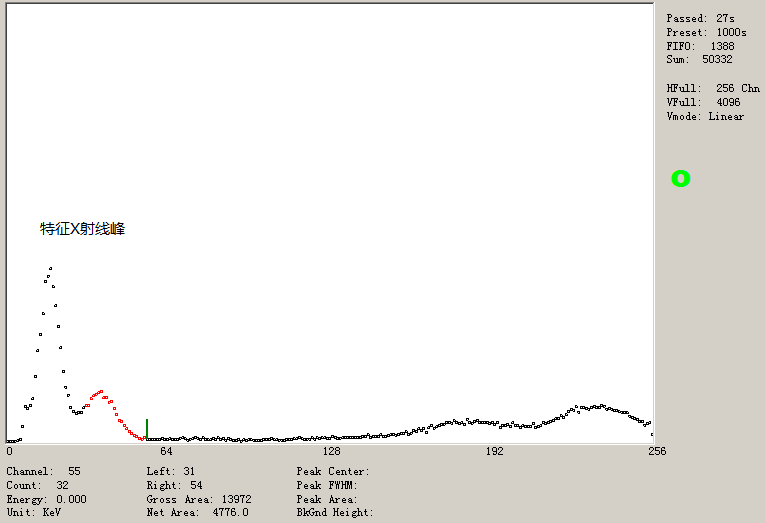
\includegraphics[width=\textwidth]{data/lowEnergy.png}
        \caption{低能部分的能谱,对应于探测器$II$}
        \label{fig:lowEnergy}
    \end{minipage}
    \qquad
    \begin{minipage}{0.45\textwidth}
        \centering
        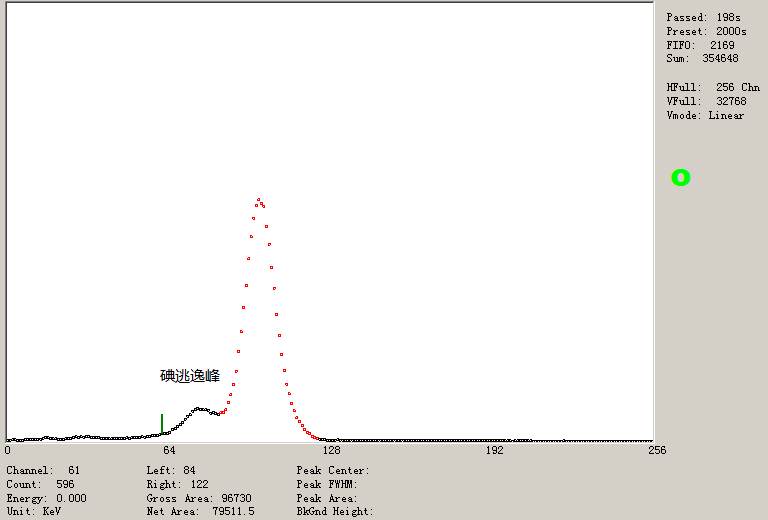
\includegraphics[width=\textwidth]{data/highEnergy.png}
        \caption{高能部分的能谱,对应于探测器$I$}
        \label{fig:highEnergy}
    \end{minipage}
\end{figure}
图~\ref{fig:lowEnergy}和图~\ref{fig:highEnergy}两个特殊的峰的位置对应的道址分别为$18,76$,而图~\ref{fig:highEnergy}中
全能峰位置在道址$100$处,与$76+18=94$较为接近,侧面验证了\texttt{碘逃逸峰}和\texttt{特征X射线}的关联。

对两个图中的特殊峰位进行阈值上的甄别,获得结果如图~\ref{fig:energyCut}
\begin{figure}
    \centering
    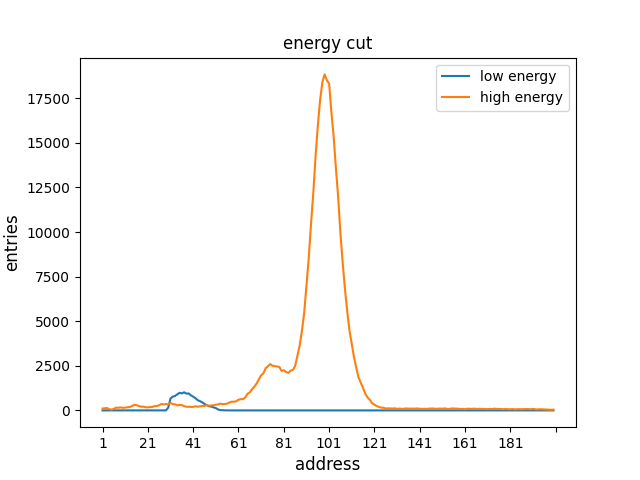
\includegraphics[width=0.8\textwidth]{data/energyCut.png}
    \caption{阈值甄别器后输出的信号结果}
    \label{fig:energyCut}
\end{figure}
\subsection{拟合原子核衰变寿命}
如图~\ref{fig:normal}中对TDC进行定标,实验采用单个信号,调节延时器件,使信号与延时信号自符合。
用线性函数对图中的点进行拟合,可以得到时间与道址之间的关系
\[t=k*x\]
\begin{figure}[htbp]
    \centering
    \begin{minipage}{0.45\textwidth}
        \centering
        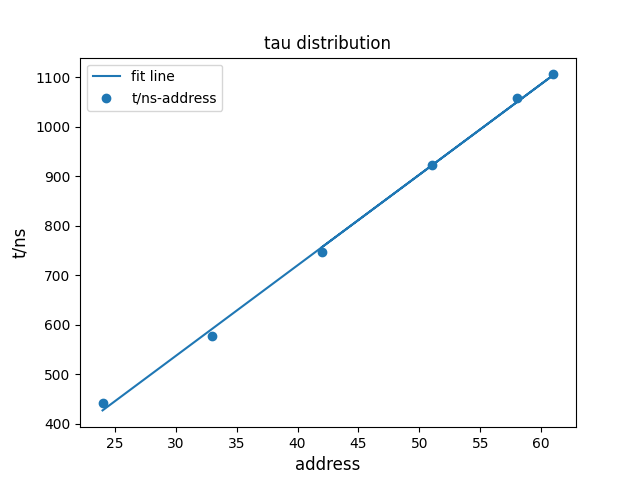
\includegraphics[width=\textwidth]{data/normal.png}
        \caption{时间标定}
        \label{fig:normal}
    \end{minipage}
    \qquad
    \begin{minipage}{0.45\textwidth}
        \centering
        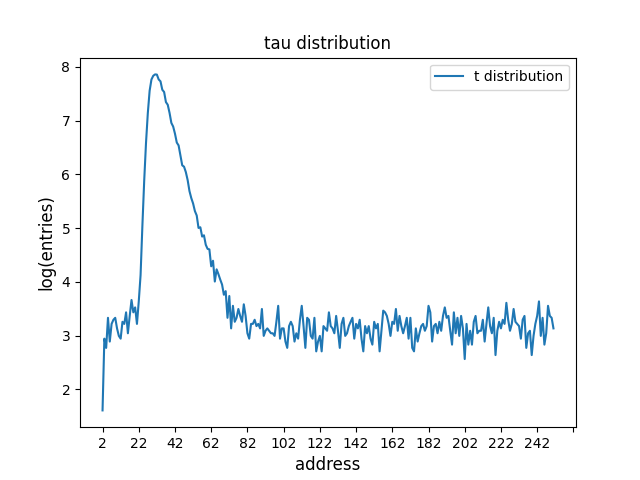
\includegraphics[width=0.8\textwidth]{data/fit.png}
        \caption{阈值甄别器后输出的信号结果}
        \label{fig:logtau}
    \end{minipage}
\end{figure}

如图~\ref{fig:taufit.png},前面部分上升,是由于,后半部分理论上服从指数分布,可以通过对于后半部分进行拟合,从而得到衰变的寿命。

本来应该对y轴取对数后使用线性函数进行拟合,如图~\ref{fig:logtau},但是前提是需要知道偶然符合计数率
\[n_{rc}=2\tau n_1n_2\]
\begin{figure}
    \centering
    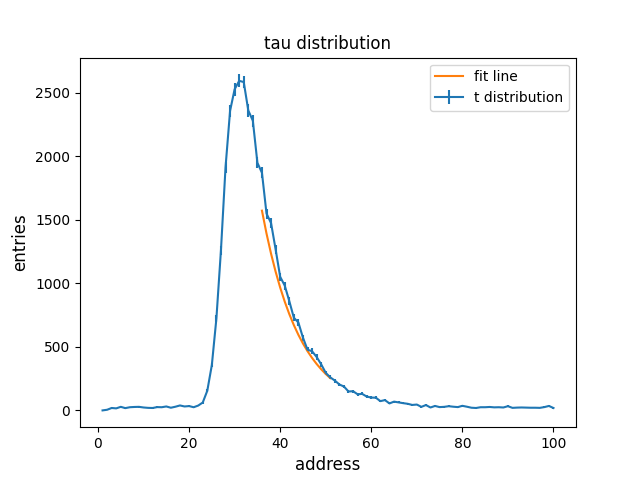
\includegraphics[width=\textwidth]{data/tau.png}
    \caption{拟合$\tau$}
    \label{fig:taufit}
\end{figure}
但是由于实验过程中忘记测量偶然符合曲线,导致无法计算出实际的$\tau$。所以图~\ref{fig:logtau}没有减去偶然符合计数率,直接取了对数,
图~\ref{fig:logtau}中仅能看出大致的线性关系。

本文采用另外一种拟合方法\texttt{likelihood}方法将偶然符合计数和
衰变寿命同时拟合出来。
\[\tau=8.229ns\]
\[n_{rc}=0\]
\section{结论}
本实验最终给出原子核衰变寿命为$\tau=8.229ns$。
\bibliography{report}
\end{document}